\documentclass{article}

\usepackage{arxiv}

\usepackage[utf8]{inputenc}
\usepackage[T1]{fontenc}
\usepackage{natbib}
\usepackage[french]{babel}
\usepackage{hyperref}
\usepackage{url}
\usepackage{booktabs}
\usepackage{amsfonts}
\usepackage{amsmath}
\usepackage{nicefrac}
\usepackage{microtype}
\usepackage{graphicx}
\usepackage{subcaption}
\usepackage{doi}

\title{Analyse Préliminaire --- Apprentissage par renforcement sur \textit{FrozenLake}}

\newif\ifuniqueAffiliation
\uniqueAffiliationtrue

\ifuniqueAffiliation
\author{
  Ibrahim R. HADJ-ARAB \\
  Faculté des sciences et de génie\\
  Université Laval\\
  \texttt{ibrahim-rabah.hadj-arab.1@ulaval.ca} \\
  \And
  Khalil EN NOUAARY \\
  Faculté des sciences et de génie\\
  Université Laval\\
  \texttt{khalil.en-nouaary.1@ulaval.ca} \\
}
\fi

\renewcommand{\shorttitle}{Analyse Préliminaire --- IFT-7201}

\hypersetup{
  pdftitle={Analyse préliminaire RL sur FrozenLake},
  pdfauthor={Ibrahim R. Hadj-Arab, Khalil En Nouaary},
}

\begin{document}
\maketitle

\noindent Code source disponible à : \url{https://github.com/Ribraba/IFT-7201-Projet}

\section{Cas d'étude}

\subsection{Composantes de l'environnement}

\textit{FrozenLake-v1}~\citep{towers2024} est un environnement de navigation en grille $N \times N$. L'espace d'états est l'ensemble des $N^2$ cases ; l'espace d'actions contient quatre déplacements (haut, bas, gauche, droite). Trois composantes peuvent être manipulées pour moduler la difficulté de l'environnement et l'exposition aux situations dangereuses :

\begin{itemize}
  \item \textbf{Degré de stochasticité.} Le paramètre \texttt{is\_slippery} contrôle la dynamique de transition. Lorsque activé, chaque action entraîne le déplacement souhaité avec probabilité $\nicefrac{1}{3}$ et l'un des deux déplacements perpendiculaires avec probabilité $\nicefrac{1}{3}$ chacun, rendant l'environnement non-déterministe.
  \item \textbf{Nombre de situations dangereuses.} Les cases de type \texttt{H} (trous) constituent les situations dangereuses. Augmenter leur nombre réduit la surface praticable et multiplie les risques de chute.
  \item \textbf{Positionnement des situations dangereuses.} Regrouper les trous de façon contiguë (ex.\ rangée horizontale) crée un obstacle de type falaise, forçant l'agent à choisir entre un chemin court risqué et un détour sûr.
\end{itemize}

La fonction de récompense est mise en forme pour accélérer la propagation du signal de danger : chute dans un trou ($r = -1{,}0$), atteinte de l'objectif ($r = +1{,}0$), collision avec un mur ($r = -0{,}1$), déplacement ordinaire ($r = 0{,}0$).

\subsection{Cas d'étude}

\begin{figure}[h]
  \centering
  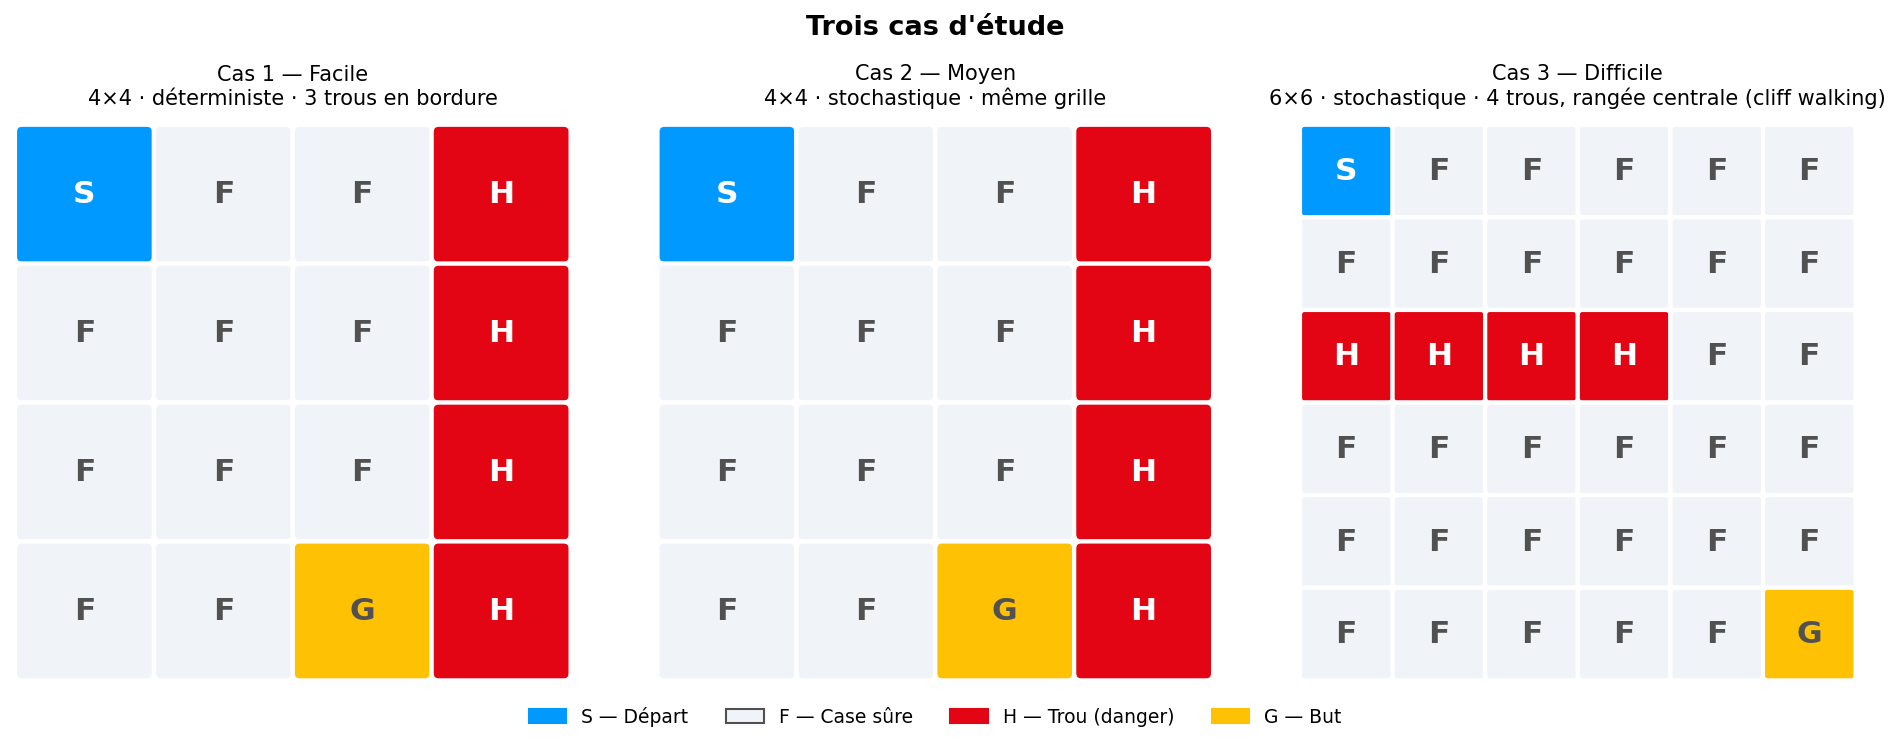
\includegraphics[width=\linewidth]{../figures/maps.png}
  \caption{Visualisation des trois environnements. \texttt{S}~: départ, \texttt{G}~: objectif, \texttt{H}~: trou (situation dangereuse), \texttt{F}~: case libre.}
  \label{fig:maps}
\end{figure}

Le Tableau~\ref{tab:configs} et la Figure~\ref{fig:maps} présentent les trois configurations retenues.

\begin{table}[h]
  \centering
  \caption{Configurations des trois cas d'étude.}
  \label{tab:configs}
  \small
  \begin{tabular}{lccc}
    \toprule
    & \textbf{Facile} & \textbf{Moyen} & \textbf{Difficile} \\
    \midrule
    Taille de la grille          & $4\times4$ & $4\times4$ & $6\times6$ \\
    \texttt{is\_slippery}        & Non & Oui & Oui \\
    Nombre de trous              & 3   & 3   & 4 \\
    Positionnement               & Colonne droite & Colonne droite & Rangée centrale \\
    \bottomrule
  \end{tabular}
\end{table}

\textbf{Facile} ($4\times4$, déterministe, 3 trous en colonne). Les transitions sont déterministes. Ce cas sert de référence : en l'absence de bruit, toute stratégie TD doit converger vers un taux de chutes nul. Il valide l'implémentation et établit une borne supérieure de performance.

\textbf{Moyen} ($4\times4$, stochastique, 3 trous en colonne). Même topologie que \textit{Facile}, mais avec \texttt{is\_slippery=True}. Ce cas isole l'effet de la stochasticité : les glissades aléatoires peuvent précipiter l'agent vers un trou même si son action choisie était sûre, quantifiant ainsi l'impact du non-déterminisme sur la sécurité durant l'apprentissage.

\textbf{Difficile} ($6\times6$, stochastique, 4 trous contigus en rangée centrale). La rangée \texttt{HHHHFF} crée une barrière partielle analogue au problème du \textit{cliff walking}~\citep[chap.~6]{sutton2018} : il existe un chemin court mais risqué longeant les trous et un long chemin sûr par les colonnes de droite. Ce cas combine les effets de la stochasticité, d'un nombre accru de trous et d'un positionnement hostile, poussant les deux stratégies à exhiber des comportements divergents face au risque.


\section{Stratégies considérées}

Deux stratégies de différence temporelle (TD) sont sélectionnées comme baselines. Il s'agit de méthodes standard ne disposant d'aucun mécanisme conçu explicitement pour éviter les situations dangereuses, ce qui permet de mesurer la limite inférieure de sécurité que tout mécanisme futur devra dépasser.

\textbf{Q-learning}~\citep{watkins1992} est une méthode \textit{off-policy} dont la règle de mise à jour repose sur la valeur maximale de l'état suivant :
\begin{equation}
  Q(s, a) \leftarrow Q(s, a) + \alpha \bigl[r + \gamma \max_{a'} Q(s', a') - Q(s, a)\bigr].
\end{equation}
Cette mise à jour optimiste suppose que la politique optimale sera suivie dans le futur, indépendamment de l'exploration en cours. Dans des environnements à obstacles groupés, cette hypothèse peut conduire à sous-estimer le risque réel de chute et à préférer le chemin court risqué.

\textbf{SARSA}~\citep{rummery1994} est une méthode \textit{on-policy} qui utilise l'action réellement sélectionnée selon la politique $\varepsilon$-greedy courante :
\begin{equation}
  Q(s, a) \leftarrow Q(s, a) + \alpha \bigl[r + \gamma\, Q(s', a') - Q(s, a)\bigr].
\end{equation}
Puisque $a'$ peut être une action aléatoire (avec probabilité $\varepsilon$), SARSA intègre le coût de l'exploration dans ses estimations. On s'attend donc à ce qu'il apprenne à éviter davantage les cases proches des trous, au prix d'une propagation plus lente du signal de danger en début d'apprentissage. La confrontation de ces deux comportements opposés face au risque est la principale motivation de leur sélection.


\section{Méthodologie expérimentale}

\textbf{Librairies.} L'environnement est fourni par Gymnasium~1.2.3~\citep{towers2024}. Q-learning et SARSA sont implémentés directement en Python/NumPy~2.2.6, sans recours à Stable-Baselines3~\citep{raffin2021}, afin de contrôler précisément les mises à jour TD.

\textbf{Hyper-paramètres.} Les deux algorithmes partagent : $\gamma = 0{,}99$ (horizon long, adapté aux trajectoires multi-étapes jusqu'à l'objectif), $\alpha_0 = 0{,}5$ (valeur standard pour les méthodes TD tabulaires~\citep{sutton2018}), décroissance $0{,}9995$ pour $\alpha$ et $\varepsilon$ jusqu'aux minima $\alpha_{\min}=0{,}01$ et $\varepsilon_{\min}=0{,}05$. Ce taux de décroissance amène $\varepsilon$ à son minimum après $\approx\!6\,000$ épisodes, assurant une phase d'exploration large suivie d'une exploitation progressive sur les 14\,000 épisodes restants.

\textbf{Paramètres expérimentaux.} Chaque configuration est entraînée sur 20\,000 épisodes, avec un maximum de 200 pas par épisode. Les expériences sont répétées avec $n=10$ graines indépendantes (graines 0 à 9) pour produire des intervalles de confiance (moyenne $\pm$ écart-type). L'évaluation finale utilise la politique greedy ($\varepsilon=0$) sur 500 épisodes.

\textbf{Indicateurs de performance.} L'étude vise à évaluer la sécurité \emph{durant} l'apprentissage et non uniquement sur la politique finale. Trois indicateurs sont mesurés :
\begin{itemize}
  \item \textbf{Taux de chutes durant l'entraînement} : fraction d'épisodes terminés dans un trou (lissé sur 500 épisodes). Mesure la sécurité au cours de l'apprentissage.
  \item \textbf{Récompense cumulée durant l'entraînement} : indicateur de convergence de la politique.
  \item \textbf{Taux d'états dangereux à l'évaluation} : fraction de pas de temps passés dans une case adjacente à un trou lors de l'évaluation greedy. Quantifie le risque de proximité avec les obstacles de la politique finale.
\end{itemize}


\section{Résultats}

\begin{figure}[ht]
  \centering
  \begin{subfigure}[t]{0.49\linewidth}
    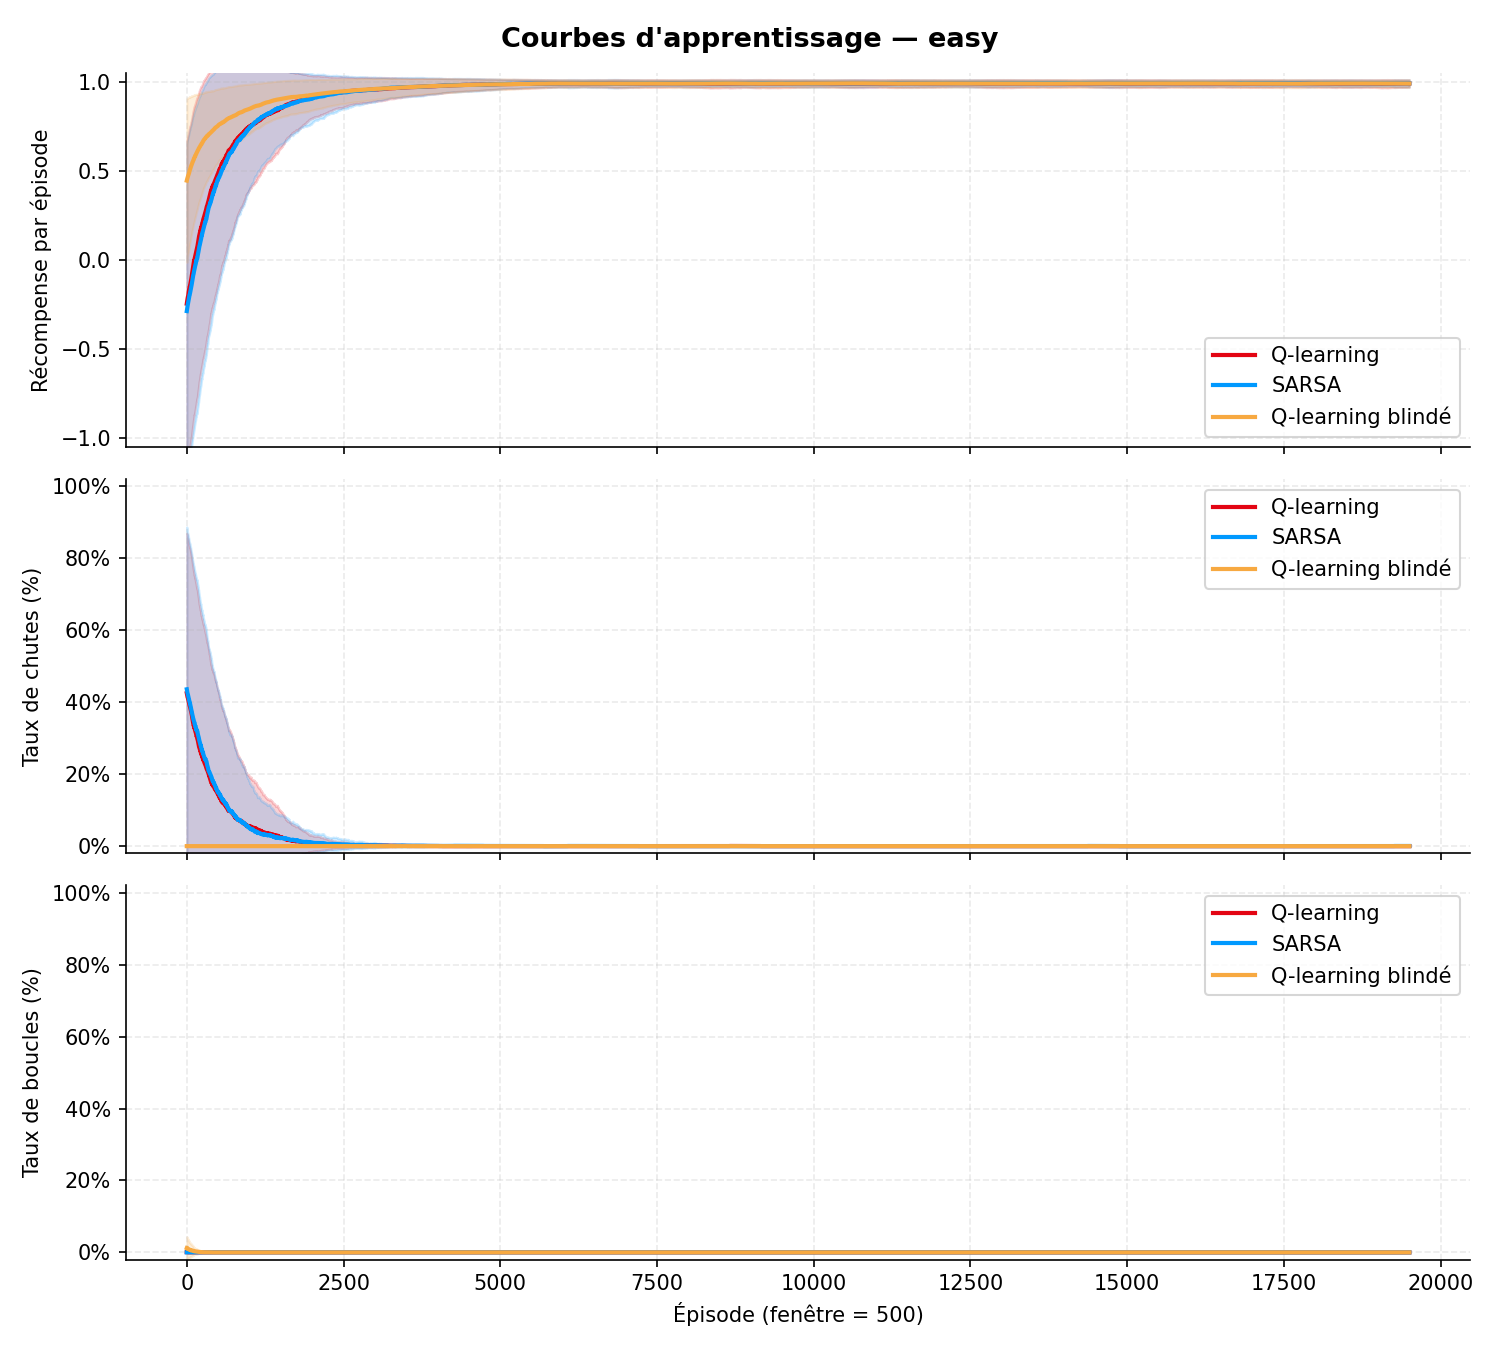
\includegraphics[width=\linewidth]{../figures/training_easy.png}
    \caption{\textbf{Facile} --- Convergence vers 0\% de chutes dès $\approx\!3\,000$ épisodes. Q-learning converge légèrement plus vite grâce à ses mises à jour optimistes. Valide les implémentations en environnement déterministe.}
    \label{fig:train_easy}
  \end{subfigure}
  \hfill
  \begin{subfigure}[t]{0.49\linewidth}
    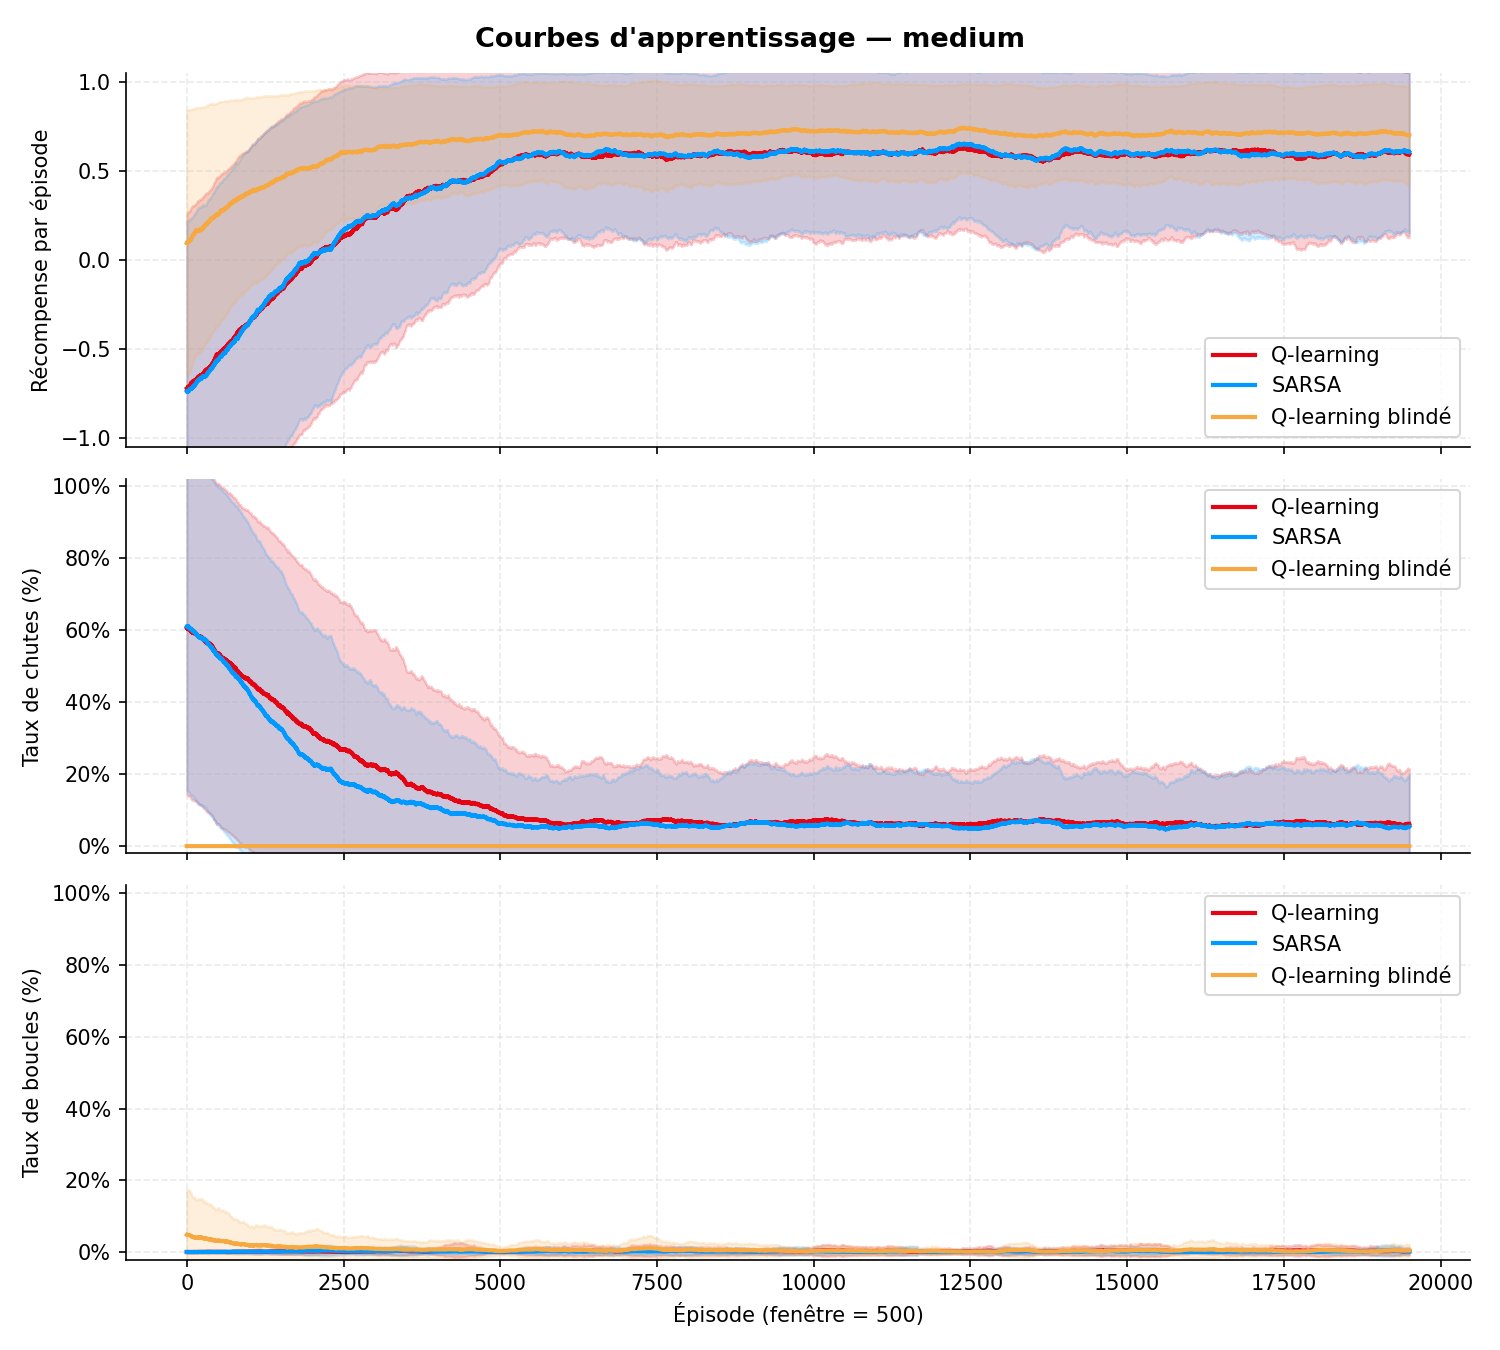
\includegraphics[width=\linewidth]{../figures/training_medium.png}
    \caption{\textbf{Moyen} --- La stochasticité fait bondir le taux de chutes initial à $\approx\!50\%$ (contre $\approx\!16\%$ en Facile). Le taux ne converge pas vers zéro : $\varepsilon_{\min}=5\%$ combiné aux glissades maintient un risque irréductible.}
    \label{fig:train_medium}
  \end{subfigure}
  \caption{Courbes d'apprentissage --- cas Facile et Moyen. La bande colorée représente $\pm$ un écart-type sur 10 répétitions.}
  \label{fig:train_easy_medium}
\end{figure}

\begin{figure}[ht]
  \centering
  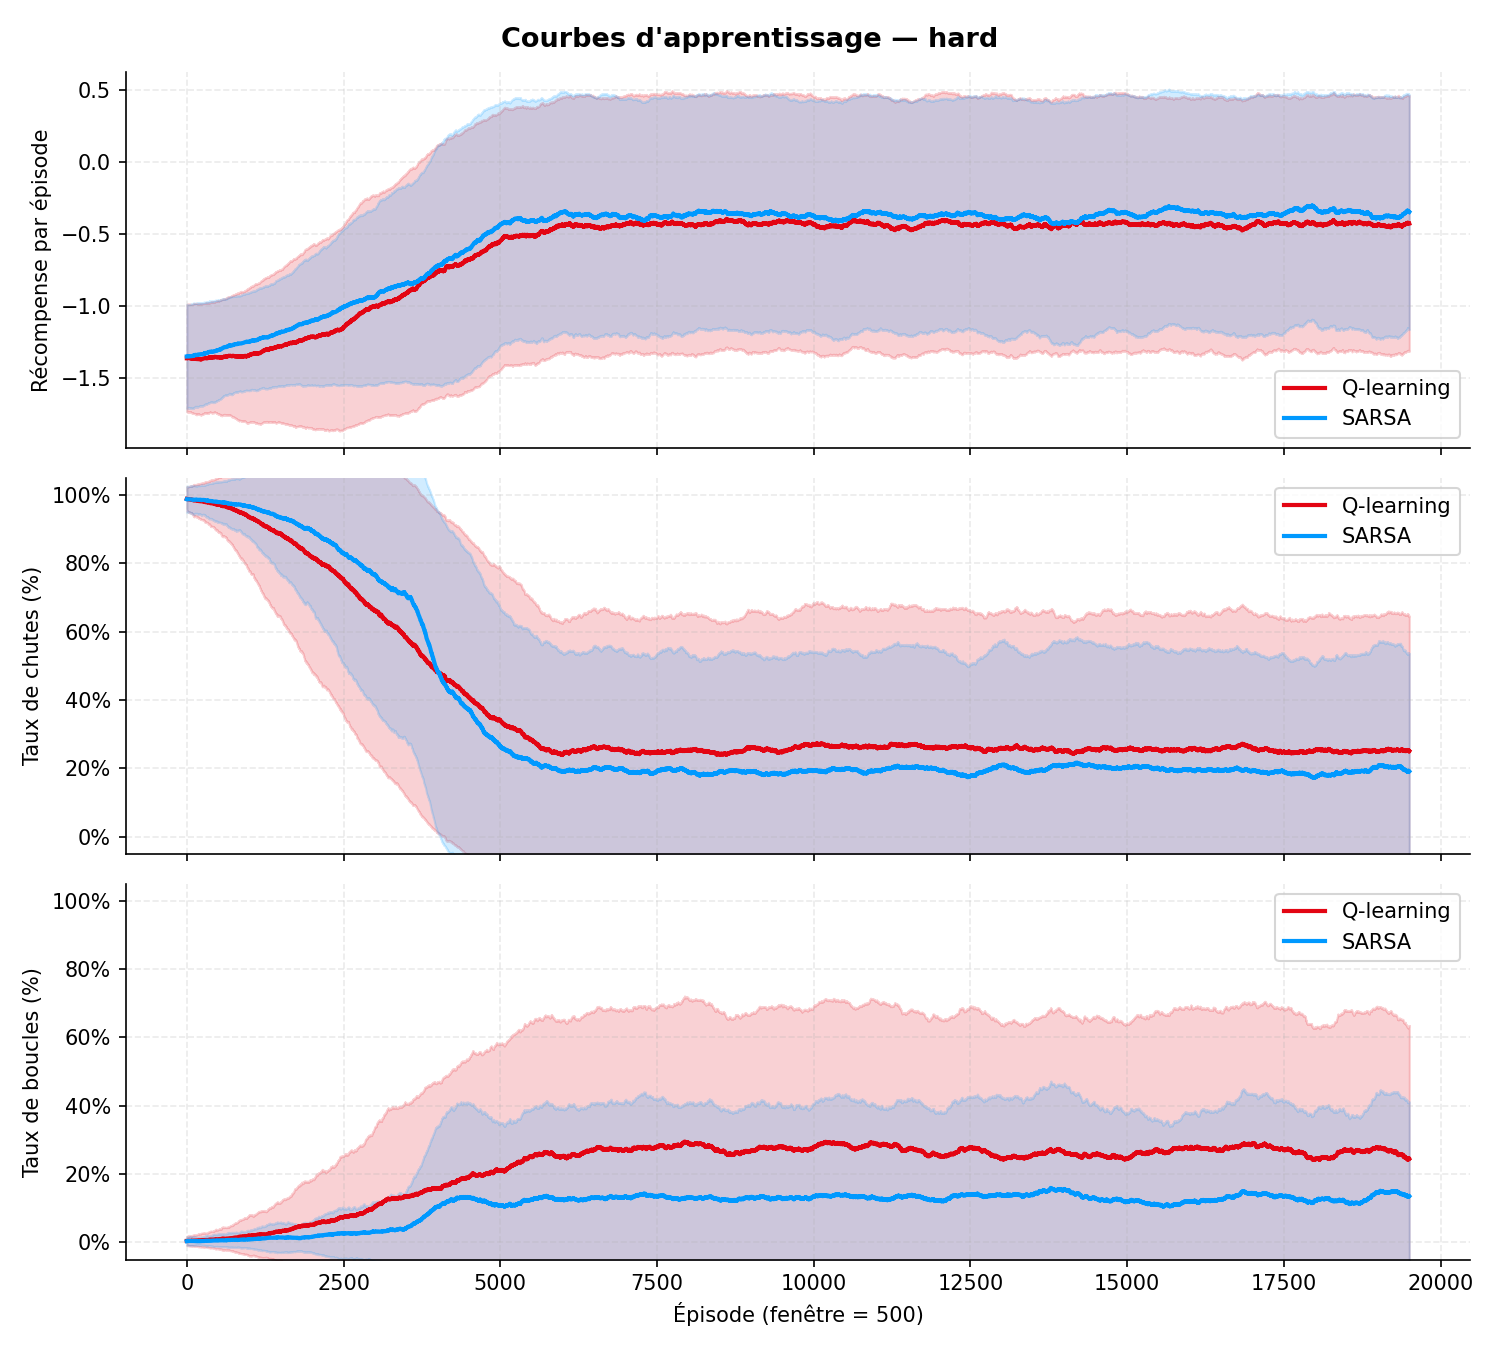
\includegraphics[width=0.7\linewidth]{../figures/training_hard.png}
  \caption{\textbf{Difficile} --- Les courbes se croisent, reproduisant le phénomène de \textit{cliff walking}~\citep{sutton2018}. SARSA chute davantage en début d'apprentissage ($94{,}1\%$ vs $91{,}3\%$) mais converge vers un taux de chutes plus faible ($15{,}2\%$ vs $19{,}9\%$) : la mise à jour \textit{on-policy} intègre le coût de l'exploration et pousse l'agent vers le détour sûr.}
  \label{fig:train_hard}
\end{figure}

\begin{figure}[ht]
  \centering
  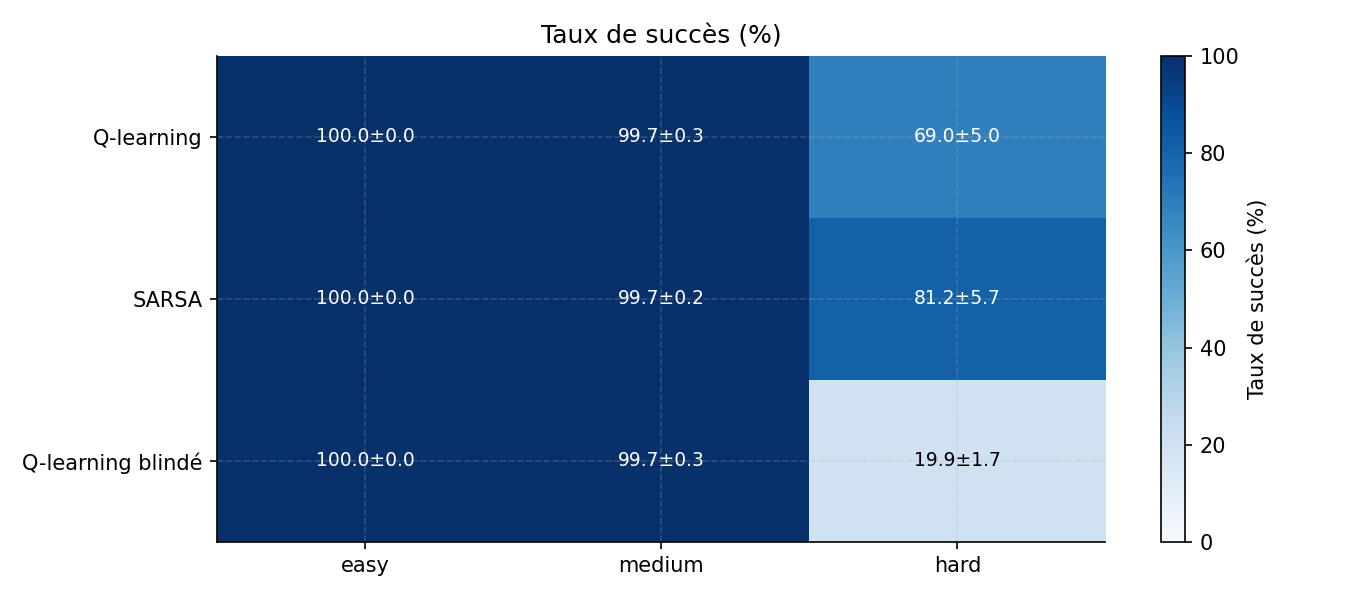
\includegraphics[width=0.7\linewidth]{../figures/overview_success_rate.png}
  \caption{Taux de succès à l'évaluation finale (politique greedy, 500 épisodes). Le taux de chutes est nul pour les deux stratégies : les échecs correspondent à des \textit{timeouts}. La comparaison de sécurité pertinente reste le taux de chutes \emph{durant} l'entraînement (Fig.~\ref{fig:train_easy_medium}--\ref{fig:train_hard}).}
  \label{fig:overview}
\end{figure}

Le Tableau~\ref{tab:danger} présente le taux d'états dangereux à l'évaluation. Sur le cas Difficile, SARSA réduit également la proximité aux trous ($27{,}4\% \pm 1{,}4\%$ contre $32{,}8\% \pm 1{,}1\%$ pour Q-learning), confirmant que son comportement plus conservateur se traduit par une politique finale qui s'écarte davantage des obstacles.

\begin{table}[ht]
  \centering
  \caption{Taux d'états dangereux à l'évaluation (moyenne $\pm$ écart-type, 10 répétitions).}
  \label{tab:danger}
  \small
  \begin{tabular}{lccc}
    \toprule
    & \textbf{Facile} & \textbf{Moyen} & \textbf{Difficile} \\
    \midrule
    Q-learning & $20{,}0 \pm 0{,}0\%$ & $28{,}5 \pm 1{,}6\%$ & $32{,}8 \pm 1{,}1\%$ \\
    SARSA      & $20{,}0 \pm 0{,}0\%$ & $27{,}7 \pm 0{,}6\%$ & $27{,}4 \pm 1{,}4\%$ \\
    \bottomrule
  \end{tabular}
\end{table}

Ces résultats montrent que Q-learning converge plus rapidement mais adopte une politique plus risquée en environnement stochastique avec obstacles groupés, tandis que SARSA, plus conservateur, réduit davantage les chutes et la proximité aux trous une fois l'exploration amortie. Ces limitations des stratégies sans mécanisme de sécurité explicite motivent l'introduction d'une telle stratégie dans le rapport final.

\bibliographystyle{unsrtnat}
\bibliography{references}

\end{document}
